\cleartooddpage
\chapter{Contribution to the DREAM Project} \label{app:dream}
\glsresetall

As part of the DREAM project, I have been involved in an international and multidisciplinary project. This led to numerous meetings and collaboration. While not presented in the main body of this thesis, I have contributed to a significant part of the software developed during the DREAM project, developed two tools to automate repetitive task tasks and contributed to papers~\citep{esteban2017build,cao2018personalized}.

\section{Software Development}

The main part of the development was focused on the architecture controlling a robot to provide therapeutic sessions for children with \gls{asd}~\citep{esteban2017build}. Workpackage 6 (Plymouth and Vrije Universiteit Brussel) was responsible to develop the robot's cognitive controller and implement the different tasks the robot would complete with the child. The overall system used the \gls{sa}: the robot suggests actions to the therapist, and the therapist can cancel them before an autonomous execution. In case of correct proposition, the therapist does not have to intervene, which leads to a reduction of the workload required for controlling the robot. An in the case of incorrect proposition, the therapist can cancel it and manually select the correct action. This ensures a therapeutically appropriate robot behaviour while not requiring the therapist to manually select each robot action. 

I was the main developer for three components: the deliberative subsystem, the expression and actuation subsystem, and the naoInterface. The deliberative subsystem was responsible to interpret steps from a script defining the session flow, to keep track of the progress in the session and to select actions that should be submitted to the teacher. Then, based on the teacher approval or selection of an action, the actuation subsystem selected the primitives corresponding to the selected  action and sent them to the robot interface. In the case of a Nao robot, the naoInterface converted these general primitives into actions executable by the robot and used the robot API (here NaoQi) the make the robot behave. 

The robot's behaviour was initially defined by human-readable scripts provided by the therapists. Part of the work was also to convert these scripts into series of steps the robot could follow. I had to interpret the therapists descriptions and translate them into logic steps including potential loops or branches (if statements). Then, I identified each simple bloc of behaviour and implemented the corresponding robot action in the deliberative, expression and actuation and naoInterface subsystems.

\section{Tools}

In addition to the components developed to run the DREAM application, I created two tools. The first one automated and simplified the use of the YARP middleware while conforming to the development standards imposed on the project, and the second one provided a human interface to create and modify the scripts used in the therapy.

\subsection{yarpGenerator}

The software development guidelines of DREAM imposed a specific folder structure for components, with a minimum number of 6 files with large overlap between components. Additionally, adding or removing one port for communication required changes in more than 10 location in 5 files. To ease this procedure, I proposed to add two new classes: the yarpInterface and the componentController. The yarpInterface class exposes all the yarp output ports required by the component to C++ functions and integrates callbacks asynchronously called when messages arrive on input ports. The yarpController is a C++ only file where code can be developed without reliance on YARP and with easy access to the input and output ports. The yarpGenerator is a tool generating automatically compilable code, complient with the development standards and including all the required files and the code to have any set of input and output ports working. Appendice~\ref{app:yarpgenerator} presents a technical report describing this tool more in depth.

\subsection{scriptManager}

The second tool provided a graphical way to read and edit the xml files describing the scripts used in the therapy scenario. This interface allows drag and drop of actions, updating parameters and copying scripts; however, no technical report is available.

\cleartooddpage
\chapter{yarpGenerator Technical Report} \label{app:yarpgenerator}
This appendix section presents the technical report corresponding to the yarpgenerator tool created for the DREAM project.

\foreachpage{appendices/yarpgenerator-guidelines.pdf}{%
	\newpage   
	\begingroup 
	\centering
	\includegraphics[
	page=\value{imagepage},
	width=\textwidth,  
	height=\textheight,
	keepaspectratio,
	]{appendices/yarpgenerator-guidelines.pdf}%
	\newpage
	\endgroup
}


\cleartooddpage
\chapter{Social Assistive Robot for Cardiac Rehabilitation} \label{app:Colombia}

A  second project I was involved in during this work was a collaboration with the Escuela Colombiana de Ingeniería Julio Garavito in Bogota. This project:  the Human-Robot Interaction Strategies for Rehabilitation based on Socially Assistive Robotics project (Royal Academy of Engineering: IAPP\textbackslash1516\textbackslash137) aimed at developing a social robot to support, monitor and assist cardiac rehabilitation for patients affected or susceptible to suffer from cardiovascular disease.

During that project, my role was to design the robot's controller. The robot guided the patients through the therapy, provided encouragements or feedback on their postures, monitored their vital signs (blood pressure, heart rate and pain level) and alerted the therapists if the patients were in a bad situation. We used a combination of preprocessed inputs and image processing with rules from the therapists to define a robot behaviour suited to this therapy. So far this collaboration contributed to two publications~\citep{lara2017human,casas2018social}, but more are being written.

\cleartooddpage
\chapter{Teacher's Diary} \label{app:diary}
This appendix section presents the daily report of the teacher's impressions and feeling when teaching the robot in the study in Chapter\ref{chap:tutoring}. It should be noted that among all the children supervised, many were special needs and as such have been removed from the result analysis. This also explains the difference of number between the children in the supervised condition (n=25) and in this diary (n=34).

%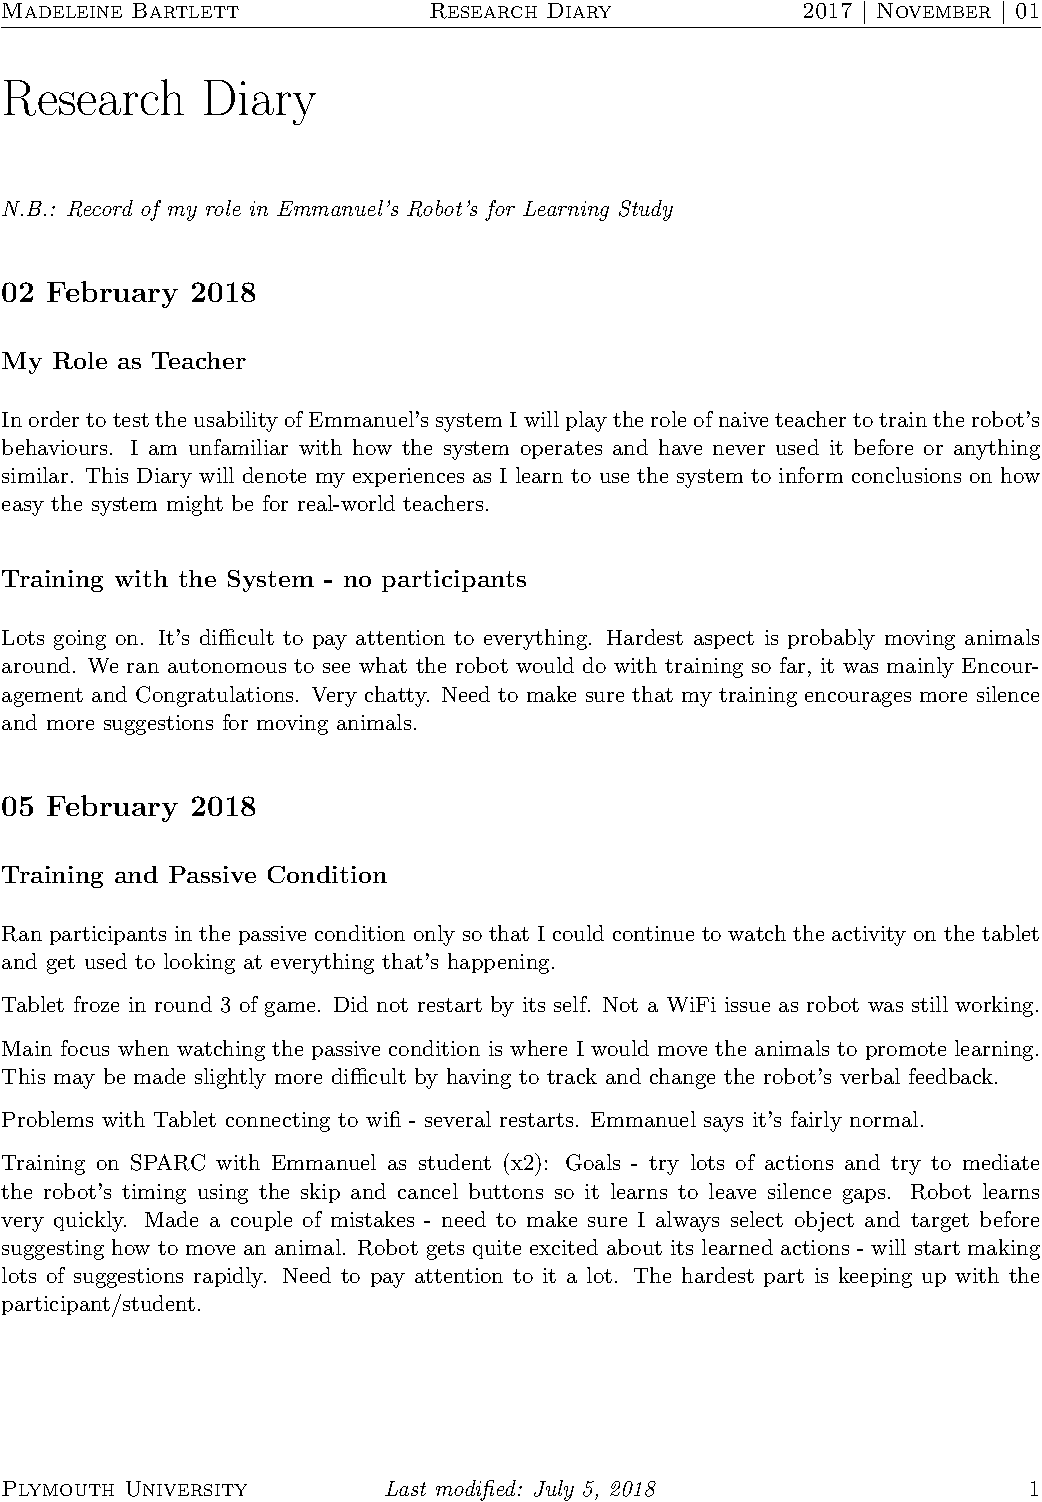
\includepdf[pages=1-14,pagecommand={},linktodoc=true]{appendices/research-diary.pdf}
\foreachpage{appendices/research-diary.pdf}{%
	\newpage   
	\begingroup 
	\centering
	\includegraphics[
	page=\value{imagepage},
	width=\textwidth,  
	height=\textheight,
	keepaspectratio,
	]{appendices/research-diary.pdf}%
	\newpage
	\endgroup
}